\documentclass[10pt,letterpaper]{article}

% page geometry

%origin
\voffset -1in
\hoffset -1in
%v
\headheight 14.5pt
\headsep 29pt
\topmargin 28.5pt
%h
\oddsidemargin 1in
%dx dy
\textwidth 6.5in
\textheight 9in

\raggedbottom
\addtolength{\topskip}{0pt plus 2\baselineskip}

% to play with
\widowpenalty=0  %1000
\clubpenalty=0 %1000
%
% and / or
%
% \setlength{\dimen0}{\textheight}
% \addtolength{\dimen0}{-\topskip}
% \divide\dimen0\baselineskip
% \setlength{\textheight}{\number\dimen0 \baselineskip}
% \addtolength{\textheight}{\topskip}
%
% or
%
 \newcommand*{\stopsection}{%
   \par
   \vspace{\fill}%
   \pagebreak[0]%
   \vspace{-\fill}%
 }
%and add \stopsection to head
\renewcommand{\stopsection}{}

%fonts
\usepackage[sc,osf]{mathpazo}
\newcommand{\lining}[1]{\fontfamily{ppl}\selectfont#1}
\newcommand{\osf}[1]{{\fontfamily{pplj}\selectfont#1}}
\usepackage{helvet}

% setup the page style
\usepackage{fancyhdr}
\lhead{\textsc{dB-SERC Course transformation}}
\chead{\textit{Project Description}}
\rhead{\textrm{Sean Garrett-Roe}}
\cfoot{\thepage}
\renewcommand{\headrulewidth}{0pt}
\renewcommand{\footrulewidth}{0pt}

\usepackage{amsmath}
\usepackage{setspace} %?
\usepackage{multirow} %for tables
 \usepackage[version=3]{mhchem} %make it use lining somehow ppl?
\newcommand{\myce}[1]{{\lining{\ce{#1}}}} %modify mhchem for OSF compatibility
\usepackage{chemnum}
\usepackage{calc} %gets the size of some text
\usepackage{microtype}
\usepackage{graphicx}
\usepackage{afterpage}
\usepackage{xspace}
\usepackage{verbatim}
\usepackage{pdfpages} %for inserting entire PDF pages?
\usepackage[numbers,sort&compress]{natbib}
%\usepackage[articletitle=true,journal=jpcbfk,sort]{achemso}

\bibliographystyle{atjvpyurl}

\usepackage[pdftex,%
    colorlinks=true,%
    urlcolor=blue,%
    citecolor=black,%
    filecolor=black,%
    anchorcolor=black,%
    linkcolor=blue%
    ]{hyperref}
\usepackage{cleveref} %must be after hyperref
\usepackage{xcolor}
%colors for highlighting
\definecolor{subheadcolor}{rgb}{0.608, 0.07,0.141} %for 154,18,36
\definecolor{arpcred}{rgb}{0.608, 0.07,0.141} %for 154,18,36
\definecolor{arpcblue}{rgb}{0,0.370,0.627} % 0,95,160
\definecolor{lowblue}{rgb}{0,0,0.75} 

\definecolor{lightyellow}{cmyk}{0, 0, .25, 0}
%\sethlcolor{lightyellow}


%figures
\usepackage{wrapfig}
\setlength{\intextsep}{.1\intextsep} %reduce whitespace around wrapfigures
\usepackage[font={footnotesize,sf},labelfont=bf,list=off,justification=raggedright]{caption}[2013/02/03] %customize captions as small san serif, bold label, and no list of figures needs to be made (which helps with internal list environments for whatever reason
\usepackage{sidecap} %figures with side captions

%lists
\usepackage[inline]{enumitem} %customize lists and inline (for captions)


%
% Set up proposal specific formatting
%
\usepackage{textcase} %for sections upper case (sc is faked in palatino right now... sigh) 
% Headings
\newcommand{\head}[1]{\stopsection\vspace{0.66\baselineskip}%
  \fontsize{11}{\baselineskip}\selectfont%
%  \noindent\textcolor{subheadcolor}{\lining{\textbf{\lsstyle \MakeTextUppercase{#1}}}}%
  \noindent\textcolor{subheadcolor}{\Large\lining{\textsc{\textbf{\lsstyle \MakeTextLowercase{#1}}}}}%
  \normalsize%
  \vspace{0.34\baselineskip}\par\nopagebreak}
\newcommand{\subhead}[1]{
\par \vspace{0.66\baselineskip}\noindent\textit{#1}\vspace{0.33\baselineskip}\par\nopagebreak}

% Aims / objectives
\makeatletter
\newcommand{\aimtext}[2]{{\color{black}\textbf{#2}}\xspace%
\immediate\write\@auxout{%
%  \string\newlabel{#1@aim}{{}{\thepage}{{\unexpanded{#2}}}{}{}}%
  \string\newlabel{#1@aim}{{{\unexpanded{#2}}{}{}}{}{}}%
}%
}

\newcommand{\aim}[1]{\stopsection\vspace{0.66\baselineskip}%
  \refstepcounter{counterAim}%
  \setcounter{counterSubAim}{0}%
  \setcounter{counterSubSubAim}{0}
  \setcounter{counterHypothesis}{0}%  
  \setcounter{counterSubHypothesis}{0}%  
  \label{#1}%
  \noindent\lining{\textbf{Specific aim \arabic{counterAim}) \ref{#1@aim}}}%
  \vspace{0.34\baselineskip}\par\nopagebreak}
%  \\*[0.34\baselineskip]\indent}
\newcounter{counterAim}
\setcounter{counterAim}{0}
\makeatother

\newcommand{\subaim}[1]{
  \refstepcounter{counterSubAim}
  \setcounter{counterSubSubAim}{0}
  \par \vspace{0.66\baselineskip}\noindent\textit{\arabic{counterAim}.\arabic{counterSubAim} #1}\vspace{0.33\baselineskip}\par\nopagebreak}
\newcounter{counterSubAim}
\setcounter{counterSubAim}{0}

\newcommand{\subsubaim}[1]{\refstepcounter{counterSubSubAim} %
%  \par \vspace*{0.33\baselineskip}\indent
  \par \indent
  \textcolor{lowblue}{%\textit{\arabic{counterAim}.\arabic{counterSubAim}.\arabic{counterSubSubAim}}
     \textit{Task \arabic{counterSubSubAim}:  #1}}}
\newcounter{counterSubSubAim}
\setcounter{counterSubSubAim}{0}
\makeatletter
\newcommand{\myssaref}{%
             \@ifstar
                  \myssarefStar%
                  \myssarefNoStar%
}
\makeatother
\newcommand{\myssarefNoStar}[1]{(\textit{Task~\ref{#1}}\xspace)}
\newcommand{\myssarefStar}[1]{\textit{Task~\ref{#1}}\xspace}

% Hypotheses
\usepackage{pifont} %access to ding
\usepackage{picture}
\newcommand{\pointer}{\begin{picture}(0,0)(\parindent,0)\put (0,0){\ding{167}}\end{picture}}
\renewcommand{\pointer}{}
\newcommand{\hypothesis}[1]{%
  \setcounter{counterSubHypothesis}{0}%  
  \refstepcounter{counterHypothesis}
  \textcolor{lowblue}{\pointer\textbf{Hypothesis \arabic{counterAim}.\alph{counterHypothesis} #1}}}
\newcounter{counterHypothesis}
\setcounter{counterHypothesis}{0}

\newcommand{\subhypothesis}[1]{ %
\refstepcounter{counterSubHypothesis} 
  \textit{\arabic{counterAim}.\alph{counterHypothesis}.\arabic{counterSubHypothesis} #1} }
\newcounter{counterSubHypothesis}
\setcounter{counterSubHypothesis}{0}


% USE CLEVEREF INSTEAD!
% reference shortcuts 
\makeatletter
\long\def\tlist@if@empty@nTF #1{%
  \expandafter\ifx\expandafter\\\detokenize{#1}\\%
\expandafter\@firstoftwo
\else
\expandafter\@secondoftwo
\fi
}
\newcommand{\myfigref}{%
             \@ifstar
                  \myfigrefStar%
                  \myfigrefNoStar%
}
\providecommand*\myfigrefNoStar[2][]{%
  (\textbf{Fig.~\ref{#2}%
\tlist@if@empty@nTF{#1}{}{, #1}% only the false code executed
})\xspace}
\providecommand*\myfigrefStar[2][]{%
  \textbf{Fig.~\ref{#2}%
\tlist@if@empty@nTF{#1}{}{, #1}% only the false code executed
}\xspace}
\makeatother
\makeatletter
\newcommand{\mytabref}{%
             \@ifstar
                  \mytabrefStar%
                  \mytabrefNoStar%
}
\makeatother
\newcommand{\mytabrefNoStar}[1]{(\textbf{Table~\ref{#1}})\xspace}
\newcommand{\mytabrefStar}[1]{\textbf{Table~\ref{#1}}\xspace}
\makeatletter
\newcommand{\myaimref}{%
             \@ifstar
                  \myaimrefStar%
                  \myaimrefNoStar%
}
\makeatother
\newcommand{\myaimrefNoStar}[1]{(\textit{Specific Aim~\ref{#1}})\xspace}
\newcommand{\myaimrefStar}[1]{\textit{Specific Aim~\ref{#1}}\xspace}


\newcommand{\caps}[1]{\textsc{\lsstyle#1}\xspace}
\newcommand{\keyword}[1]{\textbf{\textsc{#1}}}
\newcommand{\spacer}{\textperiodcentered\xspace}
\newcommand*{\ie}{\textit{i.e.},\xspace}
\newcommand*{\eg}{\textit{e.g.},\xspace}
\newcommand*{\etc}{\textit{etc.}\@\xspace}
\newcommand{\nts}[1]{}
\newcommand{\fixme}[1]{{\color{red}{\bfseries#1}}\xspace}
\newcommand{\oldtext}[1]{{\color{gray}#1}}
\newcommand{\pogil}{\caps{pogil}}
\newcommand{\recall}{\emph{retrieval}\xspace}
\newcommand{\comprehension}{\emph{comprehension}\xspace}
\newcommand{\analysis}{\emph{analysis}\xspace}
\newcommand{\use}{\emph{knowledge utilization}\xspace}
\newcommand{\Recall}{\emph{Retrieval}\xspace}
\newcommand{\Comprehension}{\emph{Comprehension}\xspace}
\newcommand{\Analysis}{\emph{Analysis}\xspace}
\newcommand{\Use}{\emph{Knowledge Utilization}\xspace}
\pagestyle{fancy}


\begin{document}
\newpage
\pagestyle{empty}
\vspace*{\fill}
\begin{center}
\head{Mastery-based grading in\\ CHEM 0110 General Chemistry 1}

\vspace{2\baselineskip}


\includegraphics[scale=1.2]{sgr_signature_2011_v2.jpg}\\
Project Director: Sean Garrett-Roe \\
\href{mailto:sgr@pitt.edu}{sgr@pitt.edu}\\
Associate Professor\\
Department of Chemistry\\
216 Eberly Hall\\
412 624 1283

\vspace{2\baselineskip}
 
Total Funds Requested: 10,000 \caps{usd}

\end{center}
\vspace{\fill}


\newpage
\pagenumbering{arabic}
\pagestyle{fancy}
\head{Abstract: Proposal overview and objectives} %<<overview>>

Student-centered pedagogies have been developed and demonstrated to improve student learning. 
For example, in the Process Oriented Guided Inquiry Learning (\pogil) approach, students construct their own knowledge
through a learning cycle of exploration, concept invention, and application.
Students progress through carefully constructed worksheets in small groups to explore a `model' (an information rich data display), answer questions that make them think about the model, propose explanations for what they have explored, and then apply those concepts to further problems.
% 
As successful as I have found \pogil to be, the assessment strategies I have used are still teacher-centered. Typical programs of high stakes assessments fundamentally undermine my learning goals for students. Rather than focusing on growing as a learner and improving as a scholar, traditional grading incentivizes a grade focus in which students try to maximize the points they can get from any assignment for the minimum of effort, independent of their learning. Poor performance on an assessment is met with the attitude that it is too late to do anything about it, so move on to the next chapter. As I result, I hate grading not because it requires effort, but because students pay no attention to the feedback and do not use the feedback as a learning opportunity. 
%work on this
The traditional grading approaches that I have used are a problem because they lead to student frustration, stereotype threat, and attrition from STEM. 

A long range goal of my teaching is to help students embrace a life of growth and learning both in the subject matter of Chemistry and in the metacognitive and metaemotional skills they need to succeed beyond the Chemistry classroom.
%
The overall objective for this proposal is to develop a mastery-based assessment structure for General Chemistry 1 that will be transferrable to other instructors in the General Chemistry program. 
% <<hypothesis>> 
The \textit{central hypothesis} is that a mastery-based grading structure -- in which questions are aligned to explicit learning objectives, student work is either proficient or not proficient (no partial credit), and students have multiple attempts at each assessment -- will better encourage and motivate students to identify their weaknesses and work to improve, leading to
% what would be better?
better learning outcomes, better attitudes about self and the subject, and a stronger growth mindset.
%
This hypothesis is based on the demonstrated effectiveness of specifications grading and standards-based grading in other General Chemistry courses.\cite{toledo2016,toledo2017,Boesdorfer2018,Martin2019}
%<<rationale>>
The \textit{rationale} of this project is that the combination of student-centered pedagogy  and student-centered assessment will synergistically improve learning outcomes for students.  These course materials will be developed with a team of General Chemistry faculty to maximize the transferability of the materials. 
%<<qualifications>>
Our team is uniquely qualified to successfully execute this project because of our experience implementing \pogil in the large-enrollment General Chemistry classroom. The specific goals for this project are to:
\begin{enumerate}[nosep,label=\textbf{\arabic*}.]
%\begin{itemize}[nosep]
\item \aimtext{aim:grading}{Develop a hierarchical set of student learning objectives aligned to a mastery-based grading scheme.} 
We will design a set of learning objectives  based on Marzano's taxonomy, which provides a structure to specify appropriate learning objectives at multiple levels of conceptual difficulty. The four tiers of achievement -- \recall, \comprehension, \analysis, and \use\ -- will be articulated for each learning objective. With this set of learning objectives, we will craft a mastery-based grading scheme that incorporates many modes of frequent, low-stakes student work.% that we already have access to -- online adaptive learning systems (Sapling Learning Curve), online homework (Sapling Learning), in-class participation (TopHat), individual and group quizzes, discussion boards.

\item \aimtext{aim:implement}{Design assessments that implement a mastery-based grading scheme.}
For each learning objective and each level of mastery, assignments will be refactored to best align with the stated learning goals. While many materials exist in the form of question banks, rarely are these questions explicitly aligned with learning objectives. We will curate materials like quiz questions and build quizzes for each learning unit. Questions will mix computer and human grading to manage the grading load to current levels. In addition,  a framework to articulate to students what learning objectives they have mastered and what areas need development will be implemented in the Canvas LMS.

\item \aimtext{aim:assess}{Assess and disseminate the course transformation.}
We will measure the impact of the transformation on student learning and attitudes. Based on our previous attitudinal data, we will compare the effect of the course on student self-efficacy and engagement, especially measures of student frustration. In addition, we will measure differential impact on students based on demographic factors such as gender. Women tend to underperform men on high-stakes assessments even though they outperform them at low-stakes assessments. We will measure student performance in the transformed course to see if it alleviates this gender bias.
\end{enumerate}
\myaimref*{aim:grading} will develop a clear, comprehensive set of learning objectives and an associated grading scheme. 
\myaimref*{aim:implement} will develop the actual assessment instruments that will assess student learning and communicate to students their progress. Finally, \myaimref*{aim:assess} will measure how effectively the course transformation has achieved each of its goals and share these results with other faculty.

This project is a \textit{creative} and \textit{original} approach to grading reform in the context of large-enrollment courses.
%
The \textit{expected outcomes} of this project will be course materials -- learning objectives, learning assessments, and course infrastructure -- whose effectiveness has been tested and is ready to be shared. 
%
\nts{The development of this project is important at several levels. First, in my classroom, these materials will help my students learn some of the hardest material better. Second, these materials can be distributed to other sections of the same course within the Department of Chemistry. Third, it will serve as a nucleus for further incorporation of active engagement aided by technology in the broader natural sciences community at Pitt. Last, validated materials can be disseminated in the \pogil community and adopted at universities around the country. }
%
Finally, this work engages a question very timely question in the broader scholarship of teaching and learning for large-enrollment courses -- how do we best build student-centered assessments that match student-centered pedagogies with our limited grading resources? 

\head{Expected significance}
This course transformation has the potential to affect many hundreds of Pitt undergraduates each term. If this transformation proves useful, other faculty in the General Chemistry teaching pool can adopt this approach beginning with the materials we will develop and share.  The transformation may also inspire other efforts to reform grading policies in other STEM disciplines through the dB-SERC community. Finally, the results of the course transformation will be disseminated in the national \pogil community.

\head{Background and preliminary results}
Guided inquiry methods~\cite{farrellJCE-99,lewisJCE-05,minderhoutBMBE-07,moog-08,eberleinBMBE-08} and Process Oriented Guided Inquiry Learning~\cite{moog-08} (\pogil) in specific, effectively bring active learning into the science classroom. Since 2012, Garrett-Roe has implemented \pogil in upper-level Physical Chemistry classes and, since 2018, in large-enrollment General Chemistry classes.\cite{Vincent-Ruz2020} As such, the \pogil pedagogy is already well-established. On the other hand, grading reform is a much newer development and a variety of approaches have been adopted. We here introduce the learning taxonomy that guides our proposed grading scheme, and introduce related grading schemes that have been demonstrated to be efficacious.

\subhead{A hierarchical taxonomy for student learning objectives}
 We are basing our  mastery-based grading scheme on a learning taxonomy with a hierarchical structure because that hierarchy more clearly articulates which tasks must be completed before progress to higher levels. This taxonomy is, naturally, very similar to Bloom's taxonomy, but we will highlight how this taxonomy guides our choices for curriculum design.

Marzano proposed a hierarchical ordering of four cognitive processes -- \recall, \comprehension, \analysis, and \use  \citep{Marzano2006}. The lowest level, \recall, focuses on the recognition or recall of information. For example, when a student is asked to define a word or provide a synonym, they demonstrate simple declarative level knowledge. The next level, \comprehension, includes integrating and symbolizing. The process of integration involves understanding general relationships in how the information is organized. For example, a student would be able to describe all variables associated with a model and the subsequent relationships between these variables. Symbolizing requires the learner to translate the knowledge into some non-linguistic or abstract form like a graph or equation. Processes that extend beyond identifying essential and non-essential characteristics of a topic fall in the domain of \analysis. An analysis task requires the learner to reorganize the information in a way that generates new conclusions. Marzano's Taxonomy proposes five processes associated with the analysis level -- matching, classifying, analyzing errors, generalizing, and specifying. Finally, the highest cognitive level, \use, includes tasks such as decision making, problem solving, experimenting, and investigating. The key distinction from analysis is the focus of the mental activity on a specific situation rather than the actual knowledge itself. For example, when a student analyzes an error involving a gas law relationship the focus is on the gas law. When the student uses a gas law to make a decision regarding whether or not to transport a container of helium gas, the focus is using the knowledge in the situation. 

\subhead{Mastery-based grading}

The grading practices of instructors generally fall into two categories -- a summative, points-based approach and a formative, mastery-based method of evaluation. The three defining characteristics of a mastery-based grading system include   \citep{Kelly2020} \begin{enumerate*}[label=\textbf{\arabic*).},nosep]
\item listing all the course content learning objectives that are assessed, 
\item awarding the
  ``mastery'' of an assignment rather than partial credit, and
  \item allowing multiple opportunities for students to achieve mastery.
\end{enumerate*}
Specific implementations of these principles are found in standards-based grading \citep{Marzano2011}, specifications grading \citep{Nilson2015}, and mastery-based testing \citep{Collins2019}. Mastery grading naturally fits with guided inquiry instruction since both are ways of promoting a growth mindset by treating knowledge and learning as an evolving process \cite{selbach2020}.

%
%Additional ideas
%
% The meaning of grades is more clear 
% It is easier to identify what students understand and what they do not

\begin{wrapfigure}{R}{0pt}
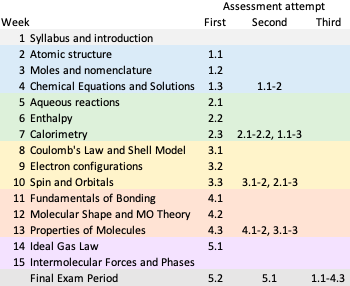
\includegraphics[width=7.5cm]{schedule.png}
\caption{\label{fig:schedule}
The working plan for the assessment schedule. Students have three opportunities to master each learning objective.}
\end{wrapfigure}

\subhead{The proposed approach}
Based on this literature, we propose to revise the assessment model of CHEM 0110 in a mastery-based approach (\cref{fig:schedule}). Each week, students will complete a learning assessment aligned to specific learning objectives for each cognitive level, \recall, \comprehension, \analysis, and \use. Preliminary learning objectives (\hyperref[app:learning_objectives]{Appendix}, \autopageref{app:learning_objectives}) and example questions (\hyperref[app:example_questions]{Appendix}, \autopageref{app:example_questions}) are provided. Every three weeks students will have another opportunity to repeat earlier assessments (\cref{fig:schedule}). Because each assessment opportunity also presents new questions, students are encouraged to participate throughout the course.

In some ways, this approach is very similar to the Quiz, Midterm, and Final model that is commonly implemented. Content units are indicated by color. Within each unit, students take two small assessments (12-15 mins, like a quiz) followed by a longer assessment ($4\times15=60$ min, like a midterm). 

On the other hand, there are important differences. Questions are clearly mapped to specific learning objectives. Student work is either proficient or not proficient -- partial credit is not awarded, but student answers do not need to be perfect to be marked proficient. The cognitive level is clearly indicated for each question. An informal analysis of exams in earlier terms of CHEM 0110 (Garrett-Roe) indicate most questions are at the \analysis level ($\sim50$), and the remainder are evenly split between \recall and \comprehension; essentially no questions reach the \use category. On the planned assessments, questions will be evenly split across these levels by design. This will help poorer performing students by providing questions that focus their attention first on the fundamentals (\recall and \comprehension), then on higher levels (\analysis and \use). Higher performing students will also be challenged by \use questions that ask them to put their understanding to work proposing, deciding, and creating.

%
% AIM Develop grading scheme and learning objectives
%
\aim{aim:grading}
Though the object of teaching is for students to learn,  the assessments used and the grading scheme applied grading often align with those learning objectives in only an intuitive, unexpressed, or traditional way. Clear-headed assessment of student learning should begin with a clear articulation of the learning objectives that is integrated into all aspects of student work and communication with students. This wholistic approach will help students identify the areas that they have mastered and the areas in which  they need to improve.

\subaim{Student Learning Objectives}
Student learning objectives that span the essential content and the hierarchy of cognitive levels from \recall to \use will be refined for the General Chemistry 1 course. Preliminary work has identified 11 major learning objectives and expressed the four mastery levels (\hyperref[app:learning_objectives]{Appendix}, \autopageref{app:learning_objectives}). These objectives will be refined to accommodate consensus among the team of \pogil instructors at Pitt. 

\subaim{Grading scheme}

\subsubaim{Levels of mastery} Four levels of content mastery are \recall, \comprehension, \analysis, and \use. Each level will be worth one point for that learning objective on a Knowledge Assessment. We will examine the feasibility of allowing students to only answer \use questions in Canvas when they have demonstrated mastery of two or three of the lower levels. 

\begin{itemize}
\item \Recall questions test simple recognition, recall, or execution of knowledge. For example, multiple choice, sorting, and multiple selection questions without significant distractors are at the \recall level. These questions likely can be computer graded. %We consider calculations that are algorithmic also to be at the \recall level.  For example,  \fixme{these questions emphasize vocabulary, definitions - no calculations} 

\item \Comprehension questions test for the integration and symbolic representation of knowledge. Multiple choice, sorting, and multiple selection questions in the presence of significant distractors that express common misconceptions are at the \comprehension level and can be computer graded. Additional questions such as explaining and drawing will likely require human graders.  

\item \Analysis questions test the ability to generate new conclusions. Many free-response calculations fall into this category. Free response numerical result questions can be computer graded. Additional proficiency in the presence of minor errors can be identified by human graders regrading select answers based on students' uploaded work.

\item \Use questions ask students to extend beyond \analysis and put their knowledge to work for their own goals. \Use questions involve steps of deciding, choosing, proposing. We anticipate that human grading will be required for all of these student responses.
\end{itemize}
Examples of questions at each of these levels are provided (\hyperref[app:example_questions]{Appendix}, \autopageref{app:example_questions}).
%
%\fixme{What level is a multiple choice calculation with significant distractors?}
%\fixme{Somewhere we need an estimate of grader time - we can balance the use of human grading for comprehension and analysis questions. Definitely necessary for use questions}

%An initial approach is given in \cref{tbl:grading_scheme_mockup}.
\begin{wraptable}{R}{0pt}
\sffamily\footnotesize
\begin{tabular}{lr}
&\textit{percent}\\
&\textit{of grade}\\
% Objective 1 & 4 &\\
% Objective 2 & 4 &\\
% $\vdots$ & &\\
% Objective 11 & 4 &\\ 
\textbf{Knowledge}&\\
\textbf{Assessments} & \textbf{55}\\
Lab  & 15\\
Homework  & 15\\
Discussion board  & 10\\
In-class participation  & *\\ 
ACS Final exam  & 5\\
Extra credit  & *
\end{tabular}
\caption{\label{tbl:grading_scheme_mockup}
The revised point structure will be quite similar to the existing point distribution.} 
\end{wraptable}

\subsubaim{Map Progress to Points} 
%We need to decide how achievement at different levels maps onto an actual score. \fixme{Is there a way to do this without taking the plunge? Estimate numbers of students at each level to keep similar grade distribution if students did similar quality work? What would we look at to evaluate if it is ok or needs to change? Seems great!}
%
We anticipate that the existing scheme for translating course points to letter grade will suffice for the course transformation. We can project how performance on the assessments will affect students' grades using typical values for performance in the other categories. Typical students will accumulate 90\% of homework, 90\% of discussion, 85\% percent lab, and 70\% on the ACS exam. The expected base score would then be 43\%. To pass the course with a C, a target of many biology students, students would need to score  54\% on the assessments, which translates to an average of 2.16 on all assessments, \ie slightly better than to achieving proficiency in all \recall and \comprehension areas. To score an A, a student would need to score 3.6 on all assessments, which corresponds to achieving proficiency in all \recall, \comprehension, and \analysis areas as well as $\sim60$\% of \use questions. 

\begin{wraptable}{R}{0pt}
\sffamily\footnotesize
\begin{tabular}{ll}
percent&Grade\\
93--99&A\\
90--92&A-\\
87--89&B+\\
83--86&B\\
80--82&B-\\
77--79&C+\\
73--76&C\\
70--72&C-\\
67--69&D+\\
63--66&D\\
60--62&D-\\
0--59&F
\end{tabular}
\caption{\label{tbl:points}
We anticipate that the scoring structure will remain unchanged.} 
\end{wraptable}

%
% AIM Implementation
%

\aim{aim:implement}

\subaim{Evaluate, revise, and write assessments}
\subsubaim{Grow a taxonomically organized question bank}\label{ssa:question_bank} Existing assessments will first be sorted by their learning outcome (subject area and cognitive level). We have a library of $\sim200$ questions that been designed in accordance with this grading scheme for human grading (Shepherd) and $\sim200$ unsorted questions that have been implemented in Canvas for automatic grading (Garrett-Roe). The pool of unsorted questions will be evaluated, grouped according to their learning level, and revised as necessary. Additional questions will be written to fill any identified gaps. We aim to develop question banks of at least $6$ questions per learning objective (264 questions total). 

% \subsubaim{Revise} Questions that are similar enough to explicit learning objectives will be revised and 

% \subsubaim{Devise} New questions will be written and put into Item Banks for sharing.

\subsubaim{Assemble assessments}
Assessments will be drafted based on the item banks developed in \myssaref{ssa:question_bank}. Each assessment will contain one question, drawn from the item banks, at each cognitive level. Item banks of 6 or more questions will provide a reasonable likelihood that students will see new questions on each attempt.

\subsubaim{Implement integration canvas}
The grade book infrastructure will be developed to calculate grades according to the grading scheme and to efficiently communicate to students their current learning progress. Potential approaches to be explored are quizzes with multiple attempts, multiple assignments with grade pooling, alignment with the Learning Objectives feature, and Mastery Paths in content Modules. We will select, from these options, the approach that offers the clearest implementation from the instructor perspective and the clearest communication to the student. Appropriate syllabus text will be developed and shared.
 
% \subsubaim{Build Grading Structure in Canvas}
% \fixme{We need to figure out a reasonable way to do this in Canvas. I am not seeing it right now. Options include \begin{enumerate*}[label=\textbf{\alph*)}]\item aligning to outcomes, \item quizzes with multiple attempts, \item an assignment group per learning objective, \item modules for each objective \item mastery paths\end{enumerate*} - Note feasibility constraints based on class size, Not sure how this differs from 2.3}

\subaim{Deploy the course transformation}
In Fall 2021, the transformed course will be implemented in the class of Garrett-Roe. Other \pogil instructors will evaluate whether or not to adopt the transformation in 2021. 

%
% AIM Assess and disseminate
%
\aim{aim:assess}
%\oldtext{some kind of introduction}

\subaim{Assess Student Learning}

\subsubaim{Course content} We will compare student performance on assessment items to 2018-2021 data.

\subsubaim{ACS General Chemistry 1 Paired Question exam.} These exams were purchased in 2018 and are available in the Department. We will compare to both national norms exam data and, perhaps more importantly, to the scores from POGIL sections in 2018 and 2019.

\subsubaim{Follow on performance} We will request support from dB-SERC to track students going into General Chemistry 2. 

%http://chemexams.chem.iastate.edu/instructors/assessment-materials/exams
\subsubaim{Student learning self-assessment}
Student perception of learning gains will be assessed through an instrument developed through \url{salgsite.org}, which provides easy implementation and analysis of the questionnaires. The question areas relevant to course learning will include
\begin{enumerate*}[label=\textbf{\arabic*.)}]
  \item how do in-class activities support learning,
\item how does the assessment structure support learning.
\end{enumerate*}

\subsubaim{Demographic effects} We will compare student performance sorted by demographic category and compare against prior years. Gender performance gaps have been identified in STEM classrooms at Pitt and suggested to be present in our Chemistry program. We will identify the magnitude of the gender performance gap in our previous General Chemistry classes 2018--2021 and compare this with student performance after the course transformation.

\begin{wrapfigure}{R}{0pt}
%\framebox[7.5cm]{
\begin{minipage}{7.5cm}
\footnotesize\sffamily
\textbf{Engagement} 
``I feel engaged during class time.'' 
\textcolor{gray}{``I do not feel engaged during class time.''} 
``I feel engaged when I am working on my homework or out of class assignments.'' 
\textcolor{gray}{``I do not feel engaged when I am working on my homework or out of class assignments.''}


\textbf{Self-efficacy}
%The attitude surveys will include questions to assess student perceptions of their self-efficacy in postively coded questions like, ``When I face a hard problem, I feel like I can solve it,'' and negatively coded questions like, ``I get frustrated easily when I face a challenging problem.'' These showed a meaningful shift after the implementation of \pogil  in the large-enrollment course compared to traditional lecture.
``When I face a hard problem, I feel like I can solve it,'' 
\textcolor{gray}{``I get frustrated easily when I face a challenging problem.''}

\textbf{Identity}
``I am a science kind of person.'' ``I am a biology kind of person.'' ``I am a chemistry kind of person.'' ``I am a physics kind of person.'' 

\textbf{Anxiety}
``I felt relaxed completing assessments (quizzes and exams).'' 
\textcolor{gray}{``Taking the assessments (quizzes and exams) was stressful.'' }
``I feel confident about my next assessment (quiz or exam).''
\textcolor{gray}{``I am worried about my performance on my next assessment (quiz or exam).'' }
%}%end framebox
\end{minipage}
\caption{Examples of positively and \textcolor{gray}{negatively} coded survey questions to assess different dimensions of student affect.}\label{fig:attitudes}
\end{wrapfigure}

\subaim{Assess Student Attitudes}
We will reimplement the assessment strategy used in the 2018-2019 terms that measured several axes of student attitudes. 
We will also capture data from concurrent \pogil and traditional lecture courses, as available. Instructors will be encouraged to offer students extra credit or some reward for participation.

\subsubaim{Questionnaires} We will use questionnaires, which can be implemented in Qualtrix, for example, to assess student attitudes. We will ask positively and negatively coded questions to measure several axes of student attitudes. We expect  dimensions to increase (self-efficacy, chemistry identity), decrease (anxiety), and not to change (engagement). 

\subsubaim{Focus groups} In addition to these quantitative surveys, qualitative data will be obtained in focus group sessions. The sessions will elicit feedback on the effectiveness of the assessment approach in the course. Sessions will be voluntary and occur at three points in the semester.

\subaim{Disseminate to Other Chemistry Faculty}
%\subaim{Feedback from \pogil faculty} 
At the beginning and end of the term of work, the \pogil Chemistry faculty (Madison, Meyer, Garrett-Roe) will meet to review the plan for the transformation and provide input into the project design. When approximately half of the course assessment material has been revised, the \pogil faculty will, as a team, review the status of the project. Feedback will be incorporated. At the end of the project, Madison and Meyer will be able to choose if they will also adopt the class transformation at this point or if Garrett-Roe will run a year as a pilot program. During the summer term, the transformation will be presented to other faculty in the General Chemistry program.

\newpage
\head{Appendices}
List of Appendices
\begin{enumerate}
%\item Departmental Letter of Support 
\item \hyperref[app:letter]{Departmental Letter of Support} (\autopageref{app:letter})
%\item Budget, Budget Justification, and Timeline 
\item \hyperref[app:budget]{Budget, Budget Justification, and Timeline} (\autopageref{app:budget})
\item \hyperref[app:learning_objectives]{Example student learning goals for General Chemistry 1 covering both subject area and level of mastery} (\autopageref{app:learning_objectives})
\item \hyperref[app:example_questions]{Examples of questions at each level of mastery} (\autopageref{app:example_questions})
\item \hyperref[app:shepherd_biosketch]{Senior staff biosketch (Shepherd)} (\autopageref{app:shepherd_biosketch})
\end{enumerate}

%\newpage
\raggedright\footnotesize\singlespacing
\renewcommand{\refname}{\large\textbf{References}}
%\renewcommand{\refname}{\Large\textsc{\textbf{\lsstyle \MakeTextLowercase References}}}
\bibliography{library_fixed,library_extra}
%trick to not typeset the bibliogrpahy but make all the data
%{\setbox0\vbox{\bibliography{library,sgr,teaching}}}

\newpage
\phantomsection\label{app:letter}
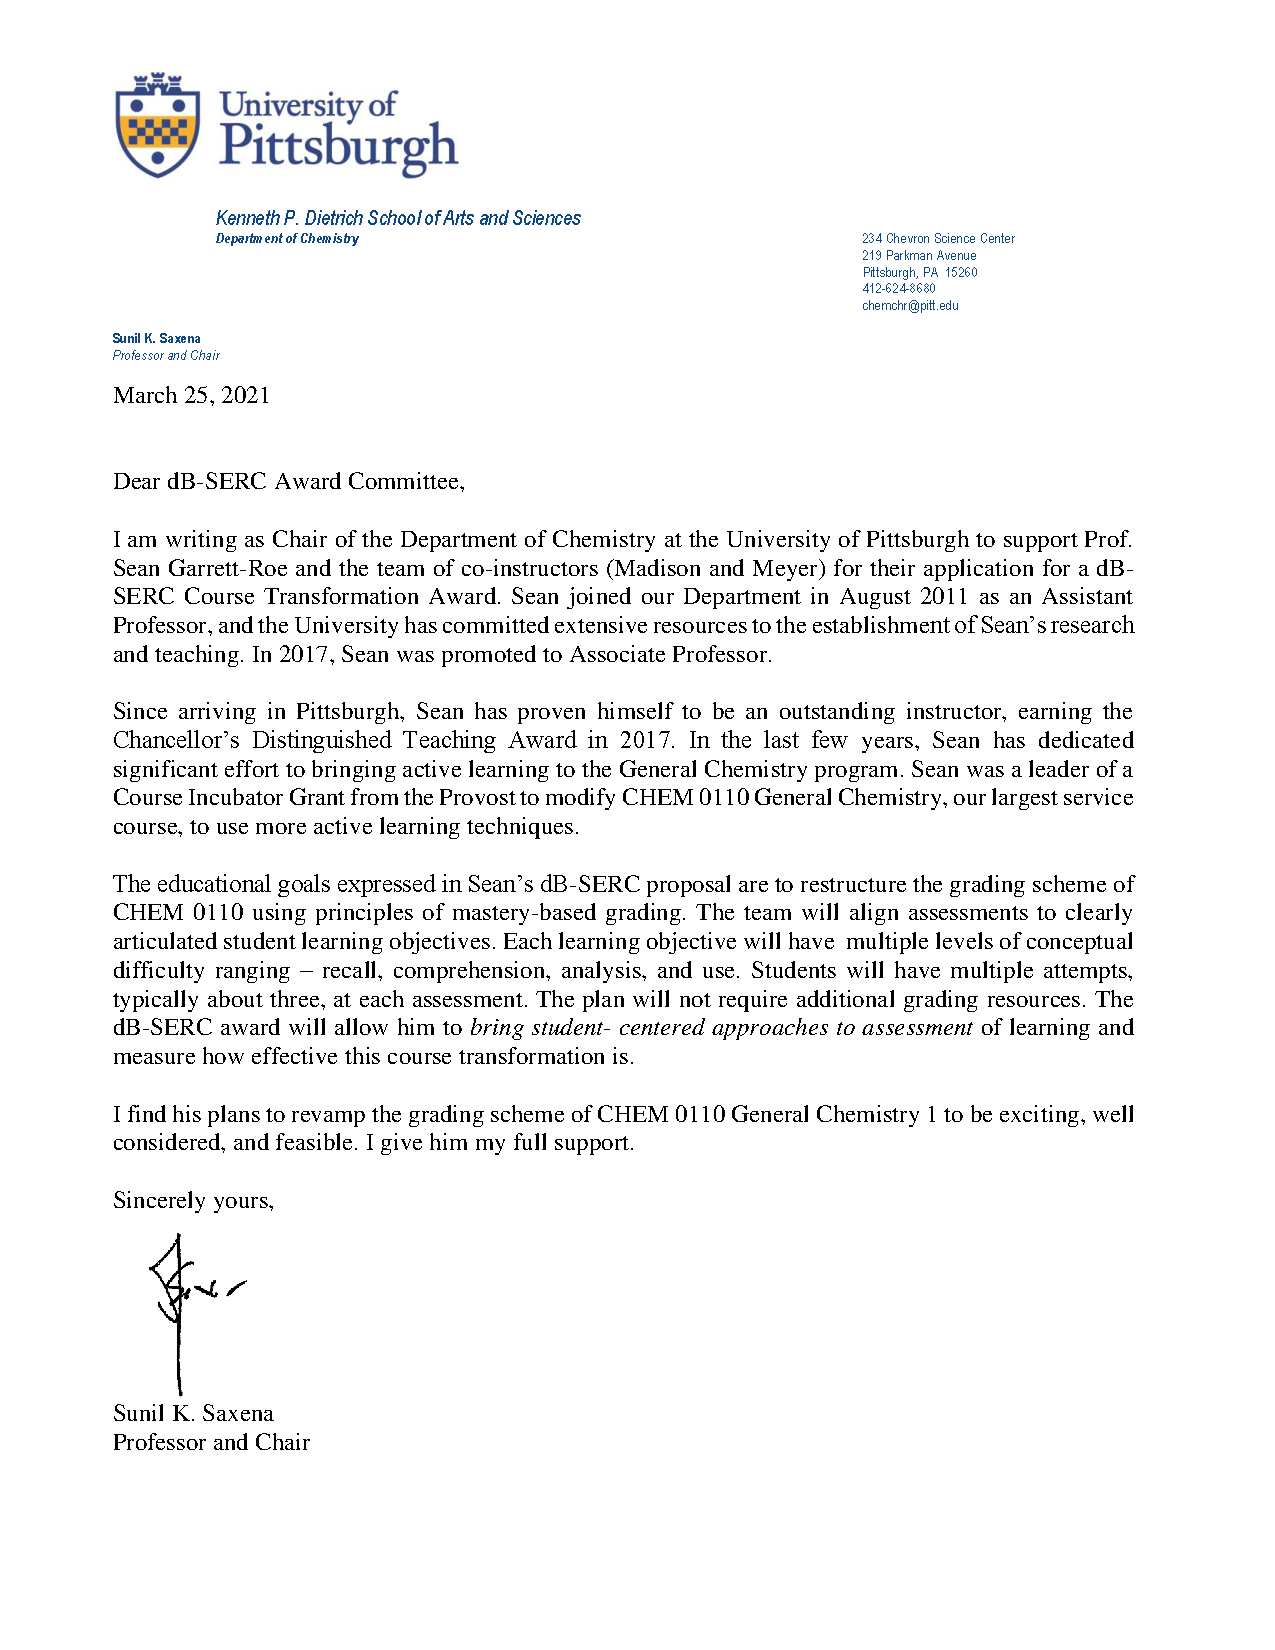
\includepdf[pages={1-},offset=75 -75]{DBSERC SGR 2021.pdf}

\newpage
\phantomsection\label{app:budget} 
%\fixme{Budget, Budget Justification, and Timeline}
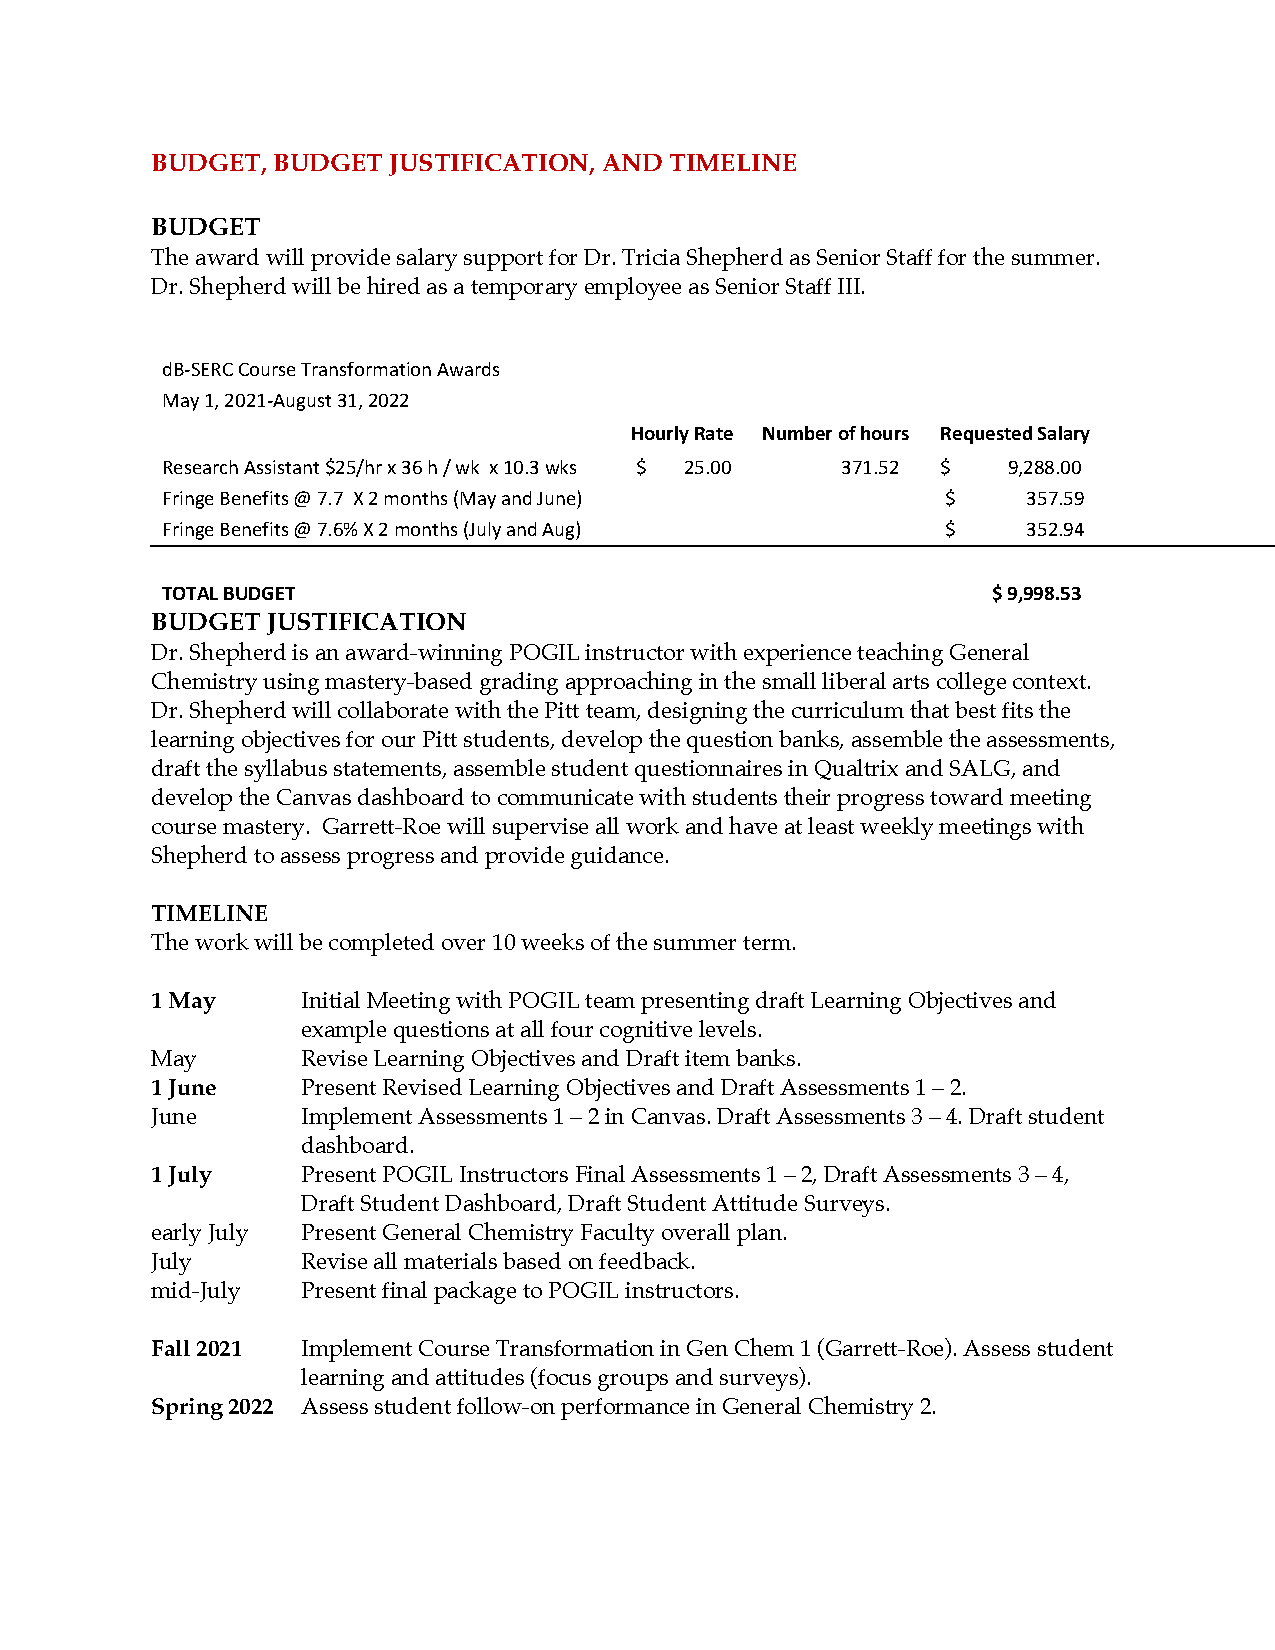
\includepdf[pages={1-},offset=75 -75]{BUDGET_Justification_Timeline.pdf}

\newpage
\phantomsection\label{app:learning_objectives}
%\fixme{PDF will go here}
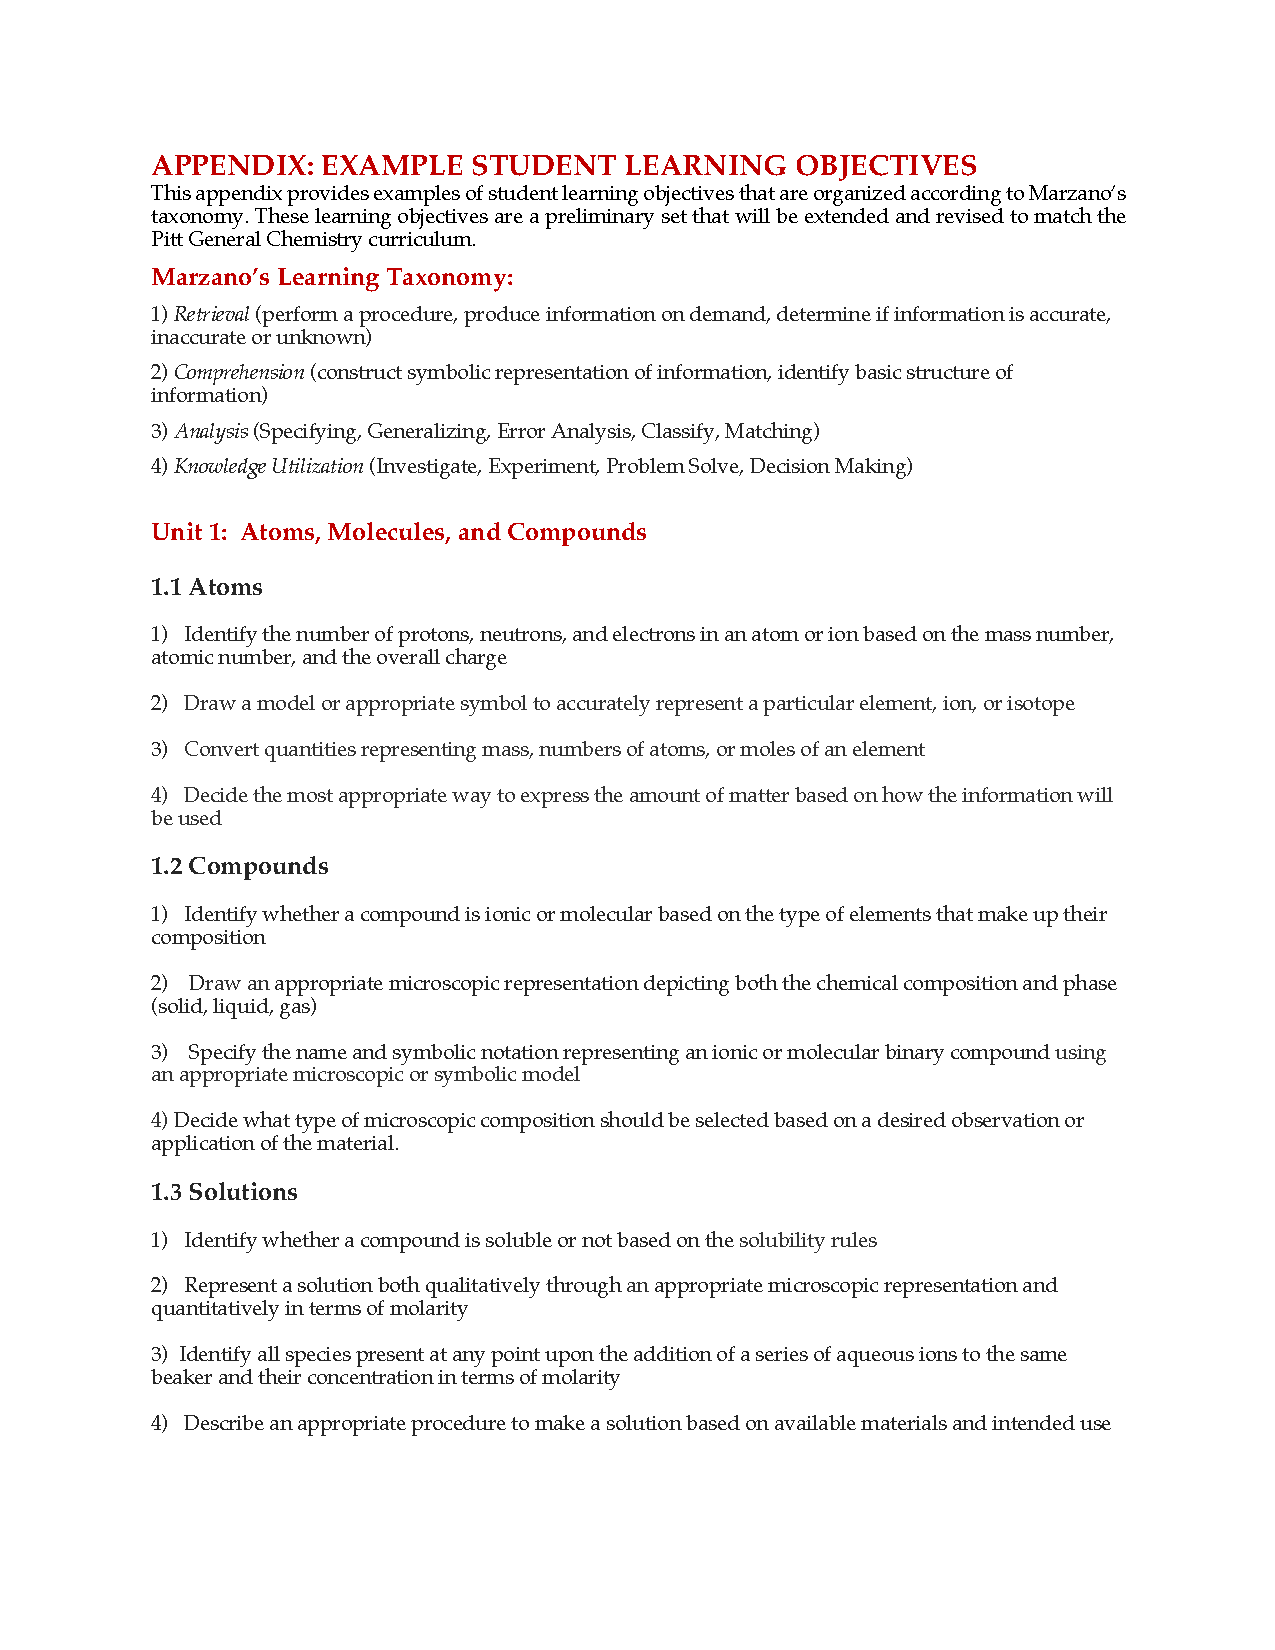
\includepdf[pages={1-},offset=75 -75]{SLOs_v2.pdf}

\newpage
\phantomsection\label{app:example_questions}
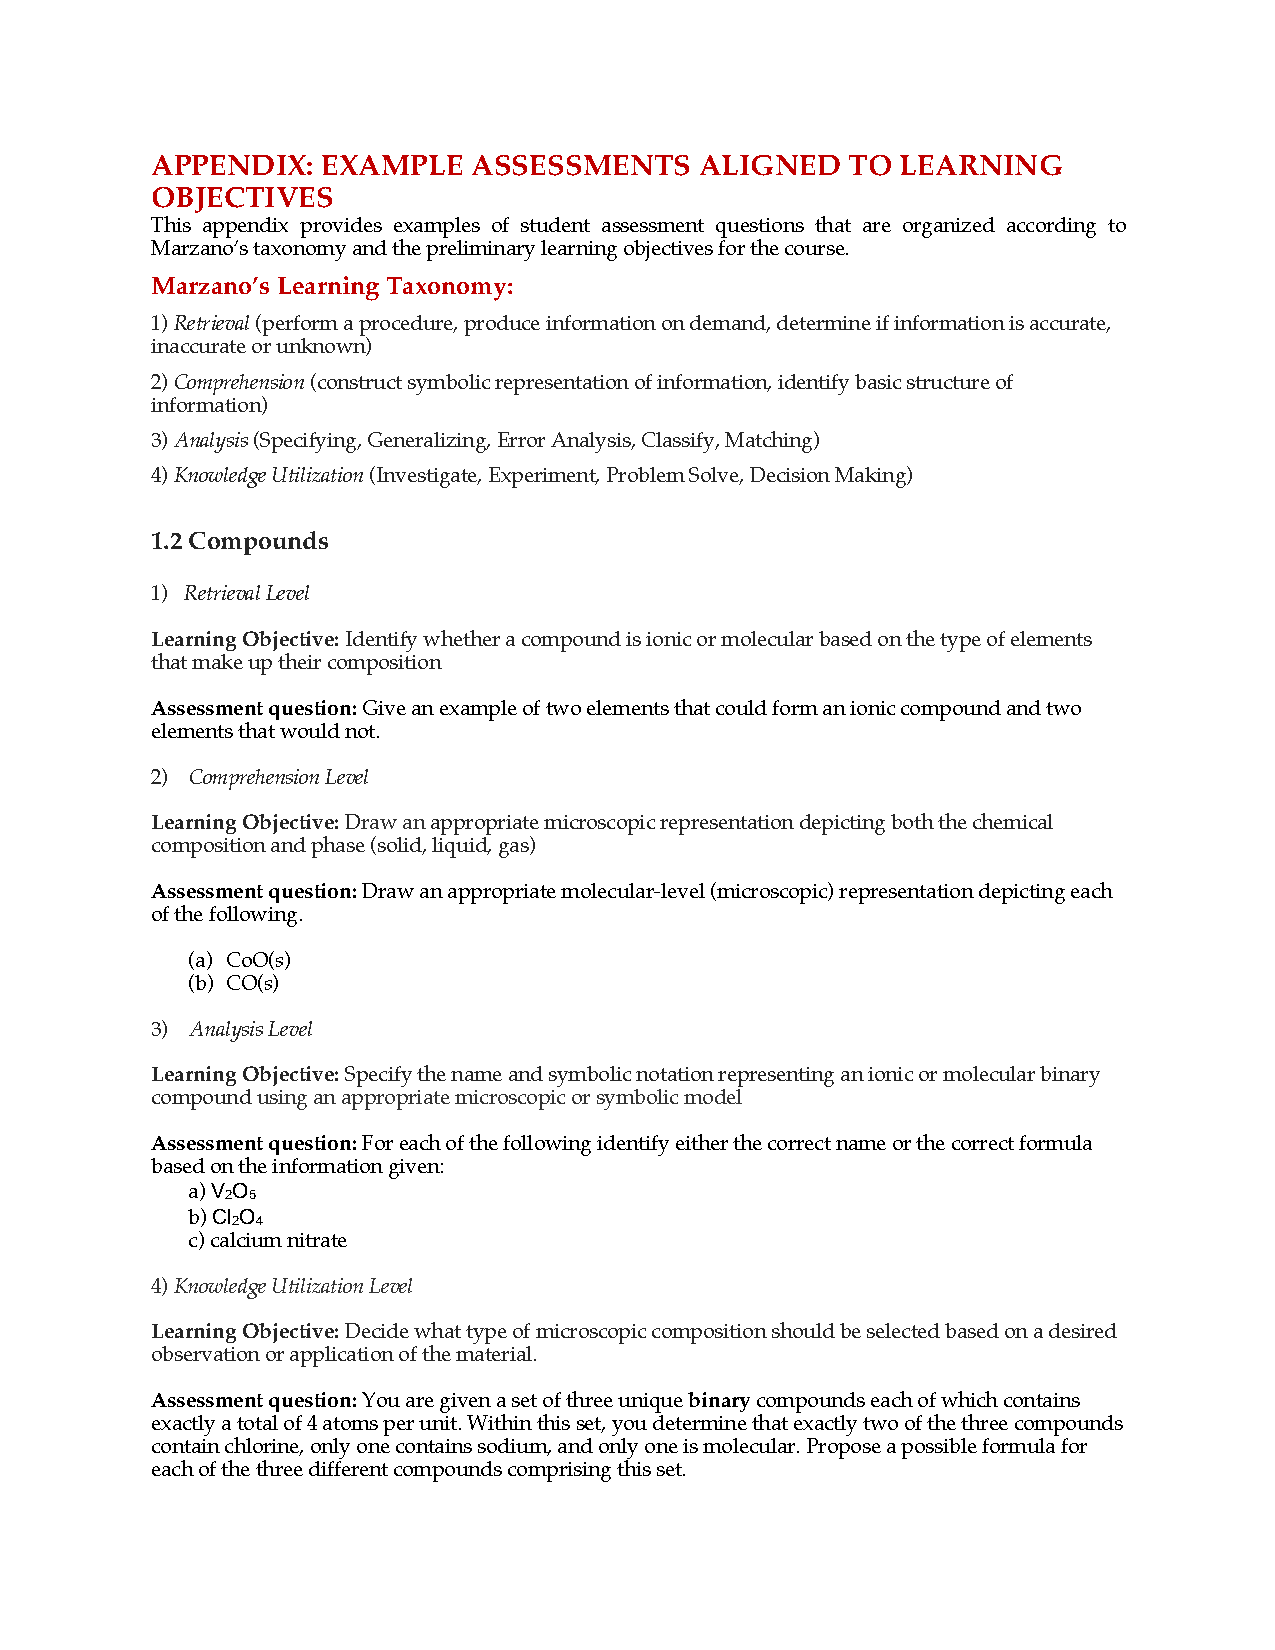
\includepdf[pages={1-},offset=75 -75]{Assessment.pdf}

\newpage
\phantomsection\label{app:shepherd_biosketch}
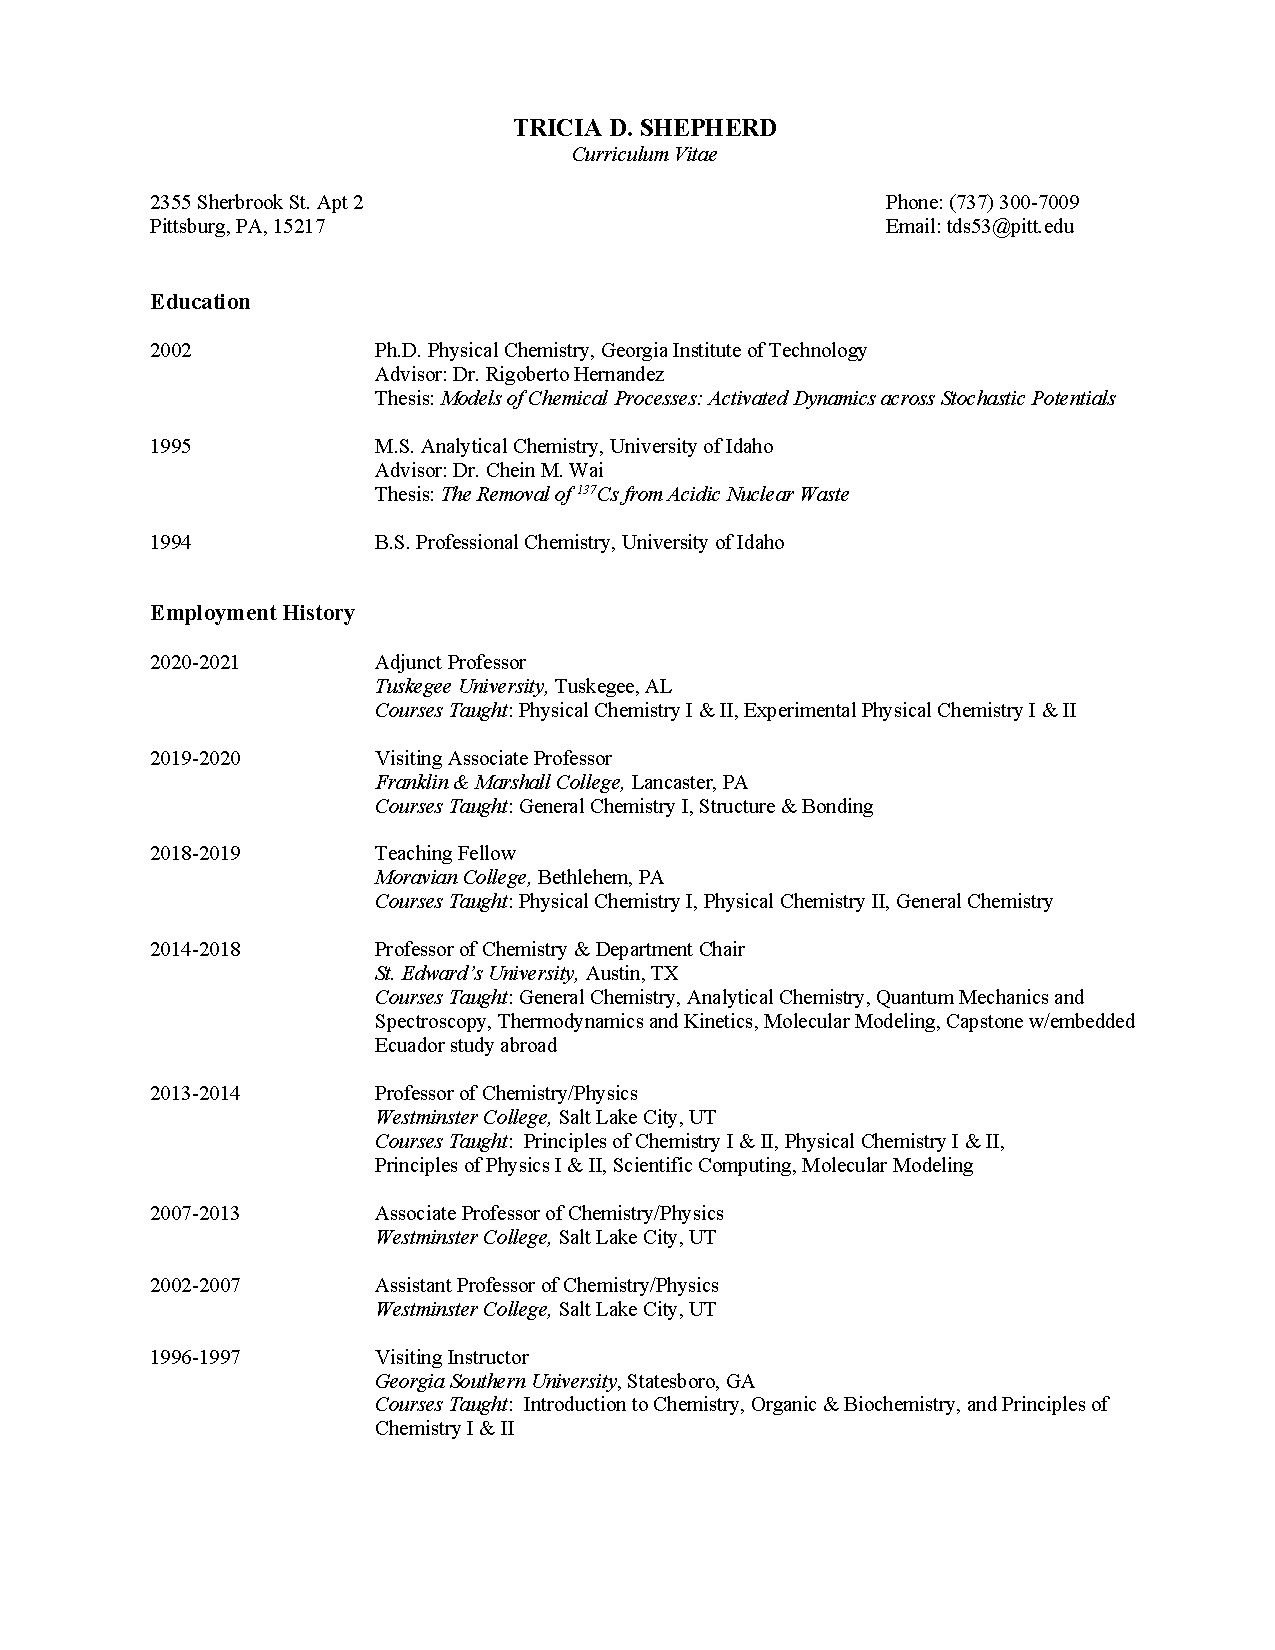
\includepdf[pages={1-},offset=75 -75]{TSCV21.pdf}


\end{document}